% Row splitting in the scalar baseline kernel, K=64 (G=8), one-column width.
% Numbers: per-thread accumulators = K^2/(32G) (FIXLOG 07-04b; 1024-thread blocks,
% R x R register tiles); K=64 -> 128 before (G=1), 16 after (G=8).
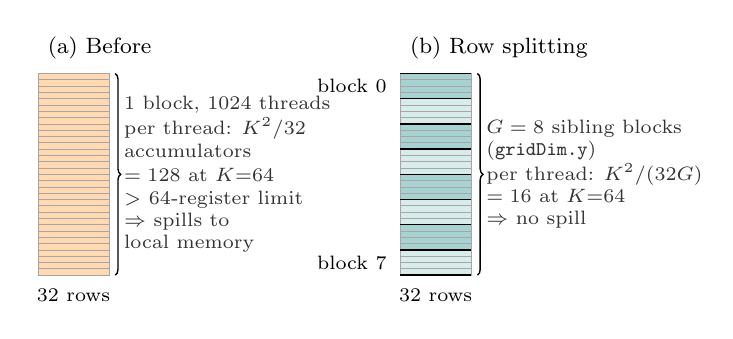
\begin{tikzpicture}[
    font=\footnotesize, x=1mm, y=1mm,
    row/.style={draw=black!35, line width=0.25pt},
    note/.style={font=\scriptsize, text=black!80, inner sep=0.8pt, align=left},
    brace/.style={decorate, decoration={brace, amplitude=2pt}, line width=0.5pt}]

% (a) defective: one block owns the whole 32-row tile row
\node[anchor=south west] at (0,27.4) {(a) Before};
\foreach \r in {0,...,31}
  \draw[row, fill=orange!30] (0,26-0.8*\r) rectangle (9,26.8-0.8*\r);
\draw[brace] (9.8,26.8) -- (9.8,1.2) node[midway, right=2.2pt, note]
  {1 block, 1024 threads\\[1pt]per thread: $K^2/32$\\accumulators\\[1pt]$= 128$ at $K{=}64$\\$>$ 64-register limit\\$\Rightarrow$ spills to\\local memory};

% (b) row splitting: G = 8 sibling blocks, 4 rows each
\node[anchor=south west] at (46,27.4) {(b) Row splitting};
\foreach \g in {0,...,7}
  \foreach \r in {0,...,3} {
    \pgfmathtruncatemacro{\shade}{mod(\g,2) == 0 ? 35 : 15}
    \draw[row, fill=teal!\shade] (46,26-3.2*\g-0.8*\r) rectangle (55,26.8-3.2*\g-0.8*\r);
  }
\foreach \g in {0,...,7}
  \draw[line width=0.5pt] (46,26.8-3.2*\g) -- (55,26.8-3.2*\g);
\draw[line width=0.5pt] (46,1.2) -- (55,1.2);
\node[font=\scriptsize, anchor=east] at (45.5,25.2) {block 0};
\node[font=\scriptsize, anchor=east] at (45.5,2.8) {block 7};
\draw[brace] (55.8,26.8) -- (55.8,1.2) node[midway, right=2.2pt, note]
  {$G = 8$ sibling blocks\\(\texttt{gridDim.y})\\[1pt]per thread: $K^2/(32G)$\\$= 16$ at $K{=}64$\\$\Rightarrow$ no spill};
\node[font=\scriptsize, anchor=north] at (4.5,0.7) {32 rows};
\node[font=\scriptsize, anchor=north] at (50.5,0.7) {32 rows};
\end{tikzpicture}
